%\documentclass[pdftex,a4paper,12pt]{article}
\documentclass[pdftex,a4paper,10.5pt]{article}

%\usepackage{graphicx}
\usepackage{float}
\usepackage[pdftex]{graphicx}
%\usepackage[latin1]{inputenc}
\usepackage[spanish]{babel}

\pretolerance=2000
\tolerance=3000

\title{\textbf{Algoritmo gen\'etico para la formaci\'on de un equipo}\\
\begin{normalsize}75.70 - Facultad de Ingenier\'ia de la Universidad de Buenos Aires\end{normalsize} }

%\author{ \textbf{Facultad de Ingenier\'ia de la Universidad de Buenos Aires}\\
%\textbf{75.70} \\ \\ 
%Ciancio Alessio, Mauro -% \textit{Padr\'on Nro. 86.357} \\
%\texttt{maurociancio@gmail.com} \\
%Gilioli, Leandro E. -% \textit{Padr\'on Nro. 86.075} \\
%\texttt{legilioli@gmail.com} \\
%L\'opez El\'ias, Lucas -% \textit{Padr\'on Nro. 85.747} \\
%\texttt{lucasdle@gmail.com} \\
%Ucciani, Juan - %\textit{Padr\'on Nro. 86.473} \\
%\texttt{jucciani@gmail.com} \\
%\texttt{njytito@gmail.com} \\
%\texttt{\{maurociancio,legilioli,lucasdle,jucciani,njytito\}@gmail.com} \\[2.5ex]
%}

\author{
	Ciancio Alessio, Mauro \and
	Gilioli, Leandro E. \and
	L\'opez El\'ias, Lucas \and
	Ucciani, Juan Manuel \and
	Yoan, Norberto \\
	\texttt{\{maurociancio,legilioli,lucasdle,jucciani,njytito\}@gmail.com}
	}
	
\date{1er Cuatrimestre de 2010}


\begin{document}
\maketitle

\begin{abstract}
	Desarrollo de una aplicaci\'on que utilice un algoritmo gen\'etico para formar un equipo para el Gran DT bas\'andose en la informaci\'on disponible de los distintos jugadores. Involucra la definici\'on de una funci\'on de aptitud para los jugadores y el uso de bibliotecas que permitan utilizar un algoritmo gen\'etico para obtener uno de los mejores equipos posibles. 
\end{abstract}

\thispagestyle{empty}
%\newpage
%\tableofcontents
%\newpage

\section{Introducci\'on}
El presente trabajo utiliza redes neuronales para la detecci\'on de figuras geom\'etricas. 
La aplicaci\'on desarrollada toma una imagen que contiene figuras (cuadrados, tri\'angulos y c\'irculos), y procesa la misma para lograr la normalizaci\'on de los datos con la finalidad de obtener entradas para la red neuronal. 
Una vez procesados los datos de entrada que representan a las figuras de la imagen, la red detecta el tipo de figura.


\section{Desarrollo}
El presente trabajo se encuentra organizado en las siguientes secciones:
\textit{Estado del arte} nos da una idea de las t\'ecnicas actuales utilizadas en aplicaciones similares en el ámbito de detecci\'on de figuras. 
\textit{Presentaci\'on del Problema} presenta el dilema a resolver.
\textit{Resoluci\'on} muestra la definici\'on de la soluci\'on planteada para resolver el problema anterior. 
\textit{Resultados} muestra luego de aplicar la soluci\'on a un conjunto de entradas que representa al espectro de entradas posibles, las diferentes salidas de la aplicaci\'on desarrollada.
Finalmente la secci\'on \textit{Conclusiones} muestra el resultado del an\'alisis del funcionamiento de la aplicaci\'on.

\subsection{Estado del arte}
El algoritmo genético es una técnica de búsqueda basada en la teoría de la evolución de Darwin, que ha cobrado tremenda popularidad alrededor del mundo durante los últimos años.
La aplicación más común de los algoritmos genéticos ha sido la solución de problemas de optimización, en donde han mostrado ser muy eficientes y confiables. Los algoritmos genéticos son de probada eficacia en caso de querer calcular funciones no derivables (o de derivación muy compleja) aunque su uso es posible con cualquier función.
Durante los últimos años una gran parte de la investigación en esta área se ha concentrado en el desarrollo de mejoras al desempeño de los algoritmos genéticos. Se han propuesto nuevas técnicas de representación, selección y cruza, con resultados muy alentadores. 
 %estado de la cuestin
%[FUMARse gugle e ieee]

\subsection{Presentaci\'on del Problema}
El problema principal que se intenta resolver es el de determinar los jugadores pertenecientes al equipo ideal para el juego del Gran DT. Uno de los mayores retos para el desarrollo de la aplicaci\'on es la de definir la forma en la que se calcular\'a la funci\'on de aptitud en base a los datos de cada jugador. Adem\'as se deber\'a integrar el c\'odigo con las bibliotecas existentes para la utilizaci\'on de algoritmos gen\'eticos y habr\'a que definir la cantidad de iteraciones o tiempo que el algoritmo realizar\'a para tener una poblaci\'on de individuos que representen un buen resultado (es decir, un buen equipo).



\subsection{Resoluci\'on}
Se encar\'o el problema dividi\'endolo en dos m\'odulos.
\begin{itemize}
\item 
M\'odulo de representaci\'on \cite{rulot}: obtiene, a partir de la imagen provista, una representaci\'on conveniente para su utilizaci\'on por el segundo m\'odulo. La tarea que realiza es el an\'alisis de la imagen de entrada en busca de blobs \cite{blobs} que luego son representados por medio de pol\'igonos de los cuales se extrae informaci\'on caracter\'istica de inter\'es que ser\'a luego alimentada al m\'odulo de la siguiente etapa.
\item
M\'odulo de interpretaci\'on \cite{rulot}: proporciona a partir del conjunto de formas u objetos presentes en la imagen y la representaci\'on convenientemente proporcionada por el m\'odulo de representaci\'on, la forma a la que pertenece el objeto, distinguiendo entre 3 posibles casos: cuadrado, tri\'angulo o c\'irculo.
\end{itemize}



Los pasos realizados por estos m\'odulos se explican a continuaci\'on:

\subsubsection{Pasos}
Para la detecci\'on de las figuras, se realiza el siguiente procedimiento:
			\begin{enumerate}
			  	\item	Se carga en memoria una imagen del archivo que se pasa como 1er
			  	argumento por l\'inea de comando. La aplicaci\'on soporta los formatos m\'as
			  	comunes (png, jpg, bmp, gif).
				\item	Se convierte la imagen a una escala de grises.
				\item 	A partir de la imagen transformada a escala de grises, se hace una
				detecci\'on de los blobs. En este paso se le especifica un umbral para el
				proceso de detecci\'on.
				\item	Se filtran los blobs detectados segun el \'area de la figura.
				\item	Con los blobs resultantes se obtienen los datos que se introducir\'an
				en la red neuronal ($ s_{1}, s_{2}, s_{3} $). Estos datos se denominan \textit{discriminantes basados en caracter\'isticas geom\'etricas} \cite{yangGillies} , y se obtienen a partir de 				           		caracter\'isticas de los blobs:
					\begin{itemize}
                      \item	Distancias promedio al punto central de los v\'ertices
                      del pol\'igono que definen al blob. Se normalizan
                      dividiendo esta distancia por la distancia al v\'ertice m\'as
                      alejado.
                      
  					  \begin{equation} s_{1} = \frac { \sum_{i=1}^{n} { {|\vec {x}_{i} - \vec{x}_{c}|^{2}} } }
				      { \max ( {|\vec{x}_{1} - x_{c}|^{2}}, ... , {|\vec{x}_{n} - \vec{x}_{c}|^{2}} ) }		\end{equation}

					  $ \vec{x}_{i}:  $	 \textit{i-\'esimo punto del pol\'igono. }
					  
					  $ \vec{x}_{c}:  $	 \textit{centroide del pol\'igono. }
						
                      \item	\'Area del pol\'igono que define el blob dividido el 
                      \'area del rect\'angulo de \'area m\'inima que contiene a ese blob.
                      
  					  \begin{equation} s_{2} = \frac { Area Blob }
				                      { Area R_{m}}		\end{equation}

					  $ R{m}:  $	 \textit{ Rect\'angulo de \'area m\'inima que contiene al Blob. }

                      \item N\'umero de v\'ertices del pol\'igono simplificado que
                      define al blob. Cuando se detecta un blob, se le pide a la
                      biblioteca utilizada un pol\'igono que define a ese blob
                      (una lista de puntos x,y). El problema que surge es que
                      esa lista contiene muchos puntos que pueden ser considerados redundantes,
                      por lo que se aplica un algoritmo \cite{ramerDouglas} para la
                      reducci\'on de los mismos que elimina los puntos que no son
                      necesarios sin deformar al pol\'igono.
                      
  					  \begin{equation} s_{3} = \frac { \#Vertices }
				                      { K  }		\end{equation}

					  $ K:  $	 \textit{M\'axima cantidad de v\'ertices para un pol\'igono simplificado. }
                      
 					\end{itemize} 
				\item   Una vez obtenidos los datos, estos son ingresados a la red neuronal
				que posee 3 neuronas de salida.
				\item La neurona que produzca el mayor valor a la salida de la red neuronal corresponde
				al tipo de figura ingresada.

            \end{enumerate}      

Se utiliz\'o una red neuronal del tipo feed-forward entrenada con back-propagation \cite{martinez}. La implementaci\'on utilizada es la que brinda la biblioteca FANN[3]. La topolog\'ia consiste en una capa de entrada con 3 neuronas, una capa oculta con 6 neuronas y una capa de salida con 3 neuronas. Estos valores fueron  definidos luego de realizar varias pruebas con diferentes topolog\'ias posibles y ver que se obten\'ia 
un buen grado de generalizaci\'on con un n\'umero reducido de neuronas. La funci\'on de activaci\'on 
elegida fue una sigmoidal.

El entrenamiento se realiza ajustando continuamente los pesos de manera que 
la salida de la red  concuerde con la salida especificada en el archivo de entrenamiento. Para 
determinar en que nivel la red se ajusta a los resultados deseados, se utiliza el cuadrado de la media 
del error, es decir, el promedio del cuadrado de la diferencia entre la salida actual y la buscada para
cada uno de los casos de entrenamiento. El ciclo se detiene cuando este valor es menor al especificado
al crear la red. Dicho par\'ametro fue probado con valores de 0.01 y 0.001, resultando este \'ultimo el 
elegido por arrojar los mejores resultados.

Para el entrenamiento de la red se utilizaron 15 casos provenientes de una imagen con 15 figuras especialmente seleccionadas para intentar cubrir un buen espectro de posibles casos.
   
             \begin{figure}[H]
	                  \begin{center}
%	                    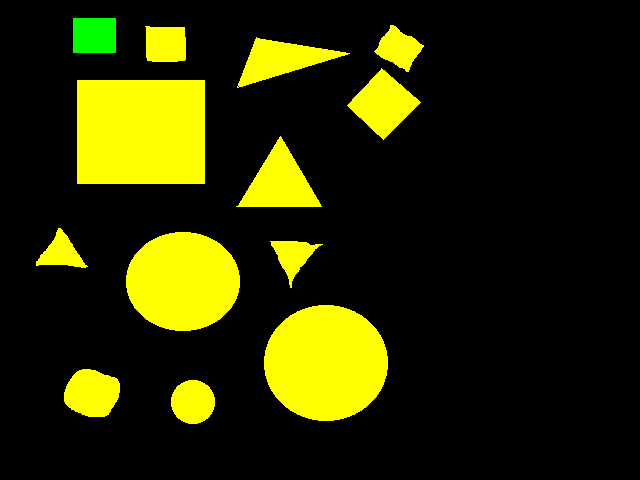
\includegraphics[width=5cm]{prueba2.png}
	                    \caption{\label{entrenamiento} Figuras utilizadas para el entrenamiento. }
	                  \end{center}
	            \end{figure}


%\includegraphics{Screenshot.png}

%incluir imagen de las figuras utilizadas para entrenar la red y quizas una tabla con los valores obtenidos

\subsubsection{Bibliotecas}
La Bibliotecas utilizadas para el desarrollo de la aplicaci\'on son las
siguientes:
\begin{itemize}

\item JGAP : es un componente de algoritmos gen\'eticos y programaci\'on gen\'etica provisto como un framework de Java. Provee mecanismos gen\'eticos basicos que pueden ser usados f\'acilmente para aplicar principios evolutivos a soluciones de un problema.

\end{itemize}
       

\subsection{Resultados} %resultados

Luego del proceso de entrenamiento de la red, se gener\'o una imagen con 27 figuras para probar el funcionamiento de la aplicaci\'on. Estas figuras presentan tama\~nos, orientaciones y geometr\'ias diversas para evaluar el grado de generalizaci\'on alcanzado.

En la figura \ref{salida_ejemlpo} se puede apreciar la salida de la aplicaci\'on en la cual puede verse el correcto funcionamiento de la misma en la gran mayor\'ia de los casos.

 	           \begin{figure}[H]

	                  \begin{center}
	                %	\advance\leftskip-1.5cm
	                  %  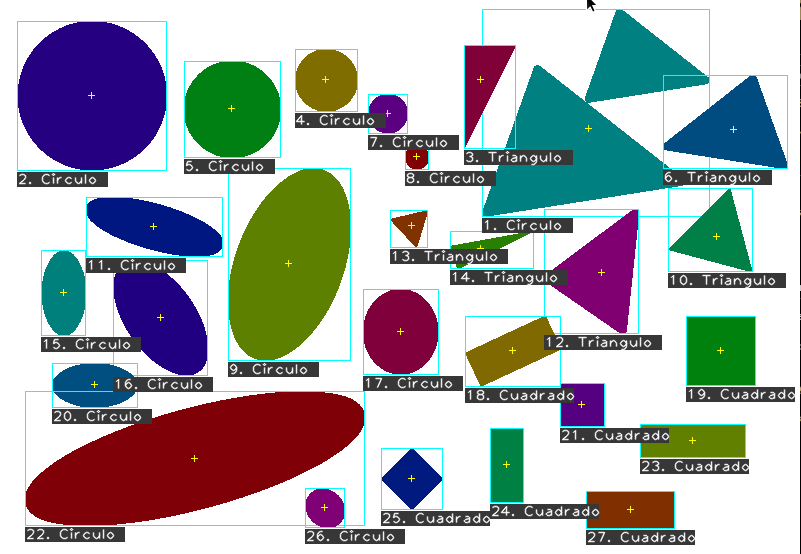
\includegraphics[width=12cm]{salida.png}
	                    \caption{\label{salida_ejemlpo} Salida generada por la aplicaci\'on. }
	                  \end{center}
	            \end{figure}

%\newpage

En la siguiente tabla se pueden apreciar algunos de los datos de entrada y salida de la red neuronal aplicada al caso de prueba presentado.

\begin{table}[ht]
\centering
\begin{tabular}{|l|c|c|c|c|c|c|c|}
  \hline                       
  \textbf{Figura} & \textbf{s1} & \textbf{s2} & \textbf{s3} & \textbf{o1} & \textbf{o2} & \textbf{o3}\\
  \hline
1 & 0.090 & 0.502 & 0.429 & -0.401 & 0.875 & 0.882\\
\hline
3 & 0.030 & 0.525 & 0.299 & 0.000 & 0.964 & -0.020\\
\hline
17 & 0.110 & 0.849 & 0.869 & -0.252 & 0.098 & 0.984\\
\hline
18 & 0.040 & 1.000 & 0.568 & 0.881 & -0.035 & 0.019\\
\hline
19 & 0.040 & 1.000 & 1.000 & 0.911 & 0.010 & 0.011\\

\hline
\end{tabular}	 
\caption{Resultados obtenidos en la corrida de prueba.}
\end{table}

\begin{flushleft}
  $ s_{i}:  $	 \textit{ Entrada de la neurona n\'umero i de la capa de entrada.}\\
  $ o_{i}:  $	 \textit{ Salida de la neurona n\'umero i de la capa de salida. }\\
  $ o_{1}:  $	 \textit{ Corresponde a un cuadrado.}\\
  $ o_{2}:  $	 \textit{ Corresponde a un tri\'angulo.}\\
  $ o_{3}:  $	 \textit{ Corresponde a un c\'irculo.}\\
\end{flushleft}

	        

\newpage
\subsection{Conclusiones} %conclusiones

	En base a los resultados obtenidos, al proceso de desarrollo de la aplicaci\'on y
	entrenamiento de la red podemos elaborar las siguientes conclusiones:
	
	La preparaci\'on de los datos result\'o ser la tarea de mayor complejidad y clave para
	lograr buenos resultados en el reconocimiento. Esto incluye la definici\'on de los atributos
	discriminantes que permitan distinguir a la red entre los distintos tipos de figuras.
	
	Por otro lado, las bibliotecas preexistentes en el mundo del software libre orientadas
	al procesamiento de im\'agenes facilitan la tarea de preparaci\'on y procesamiento 
	de los datos.

	Existen una gran cantidad de herramientas, y el desaf\'io se encuentra en encontrar
	la m\'as adecuada y madura para realizar la tarea deseada.

	La elecci\'on del tipo de red neuronal y la definici\'on de los aspectos antes mencionados
	fue apropiada ya que se obtuvo un alto grado de precisi\'on como puede observarse
	en los resultados expuestos.
	
	El tama\~no de la red no result\'o tan importante como la definici\'on de sus par\'ametros.

\section{Posteriores l\'ineas de Investigaci\'on} %Nuevas lineas de investigacin que se nos fueron ocurriendo

Al presente sistema se le podrían realizar las siguientes mejoras:

\begin{itemize}

\item  Utilización de operadores dinámicos, esto implica que los operadores se modifiquen durante
la ejecución del proceso, por ejemplo, el operador de mutación podría incrementar o reducir
su porcentaje de incidencia en función al resultado que se va obteniendo durante la corrida
del sistema.
\item Modificación de la función de aptitud para incluir m\'as restricciones, el sistema podría tener otros componentes y funcionar en base a otras variables. 
\item Modificar el operador de selección.
\item Expandir la utilización del sistema a otras áreas.

\end{itemize}
\newpage

\begin{thebibliography}{9}

\bibitem{martinez}
 García Mart\'inez,
 \emph{Algoritmos Gen\'eticos}.
 Centro de Ingenier\'ia del Software e Ingenier\'ia del Conocimiento
 Instituto Tecnológico Buenos Aires. 

\bibitem{Cantu-Paz}
 Cant\'u-Paz,
 \emph{A Summary of Research on Parallel Genetic Algorithms}.
 IlliGAL Report No. 95007, University of Illinois
 Julio 1995

\bibitem{De Jong}
 De Jong, Spears,
 \emph{A Formal Analysis of the Role of Multi-Point Crossover in Genetic Algorithms}.
Annals of Mathematics and Artificial Intelligence Joumal,
 Vol 5, No. 1, 1992

\bibitem{Goldberg}
 Goldberg,
 \emph{Genetic Algorithms in Search, Optimization, and Machine Learning}.
 Addison-Wesley Publishing Company
 1989
 
\bibitem{Goldberg2}
 Goldberg,
 \emph{Genetic and Evolutionary Algorithms}.
 Age Communications of the
 ACM, Vol. 37, No. 3, 
 Marzo 1994

\bibitem{Goldberg3}
 Goldberg,
 \emph{Genetic Algorithms, Selection Schemes, and the Varying Effects of Noise}.
 IlliGAL Report No. 95009, 
 University of Illinois, 
 1995
 
\bibitem{Spears}
 Spears,
 \emph{Crossover or Mutation}.
 Proceedings of the Foundations of Genetic Algoritluns Workshop Vail, Colorado, pag. 221- 237,
 Julio 1992
 
 \bibitem{jgap}
 JGAP, 
 \emph{Genetic Algorithms and Genetic Programming package}
 Release: 3.4.4,
 Octubre 2009
 

\bibitem{Holland}
 Holland,
 \emph{Schemata}.
  GA-List, GA Vol. 8 No. 26,1994 [MIL/95]
  
\bibitem{Miller}
 Miller,Goldberg, 
 \emph{Genetic Algoriduns, Toumwnent Selection, and the Effects of Noise}.
 IlliGAL Report No. 95006, University of Illinois, 1995
  

  
\end{thebibliography}

%No tiene que tener menos de 7 hojas ni mas de 10
%y en A4 abrochado.
%formato paper.

\end{document}
